

\documentclass[10pt,a4paper,twoside]{article}
\usepackage[dutch]{babel}
\usepackage{amssymb}
\usepackage{amsmath}
\usepackage{float,flafter}	
\usepackage{hyperref}
\usepackage{inputenc}
\setlength\paperwidth{20.999cm}\setlength\paperheight{29.699cm}\setlength\voffset{-1in}\setlength\hoffset{-1in}\setlength\topmargin{1cm}\setlength\headheight{12pt}\setlength\headsep{0cm}\setlength\footskip{1.131cm}\setlength\textheight{25cm}\setlength\oddsidemargin{2.499cm}\setlength\textwidth{15.999cm}
\begin{document}
\begin{center}
\vspace{.3cm}
{\bf {\huge Term paper}}
\item
{\bf {\huge ORM in DBMS}}
\vspace{.3cm}
\end{center}
{\bf Name:} Bhavin Raichura\\
{\bf Roll no:} 19111019 \\
{\bf Subject:} DBMS\\
{\bf Branch:} Biomedical Engineering \hspace{\fill}   \\
\hrule

\vspace{.5cm}
\vspace{.4cm}

\renewcommand{\abstractname}{Abstract}

\begin{abstract}
\item One of the challenges of using object-oriented programming (OOP) languages and databases is the complexity of aligning the programming code with database structures. Object-relational mapping (ORM) is a technique that creates a layer between the language and the database, helping programmers work with data without the OOP paradigm.
\item The necessity to learn and code in structured query language (SQL) in order to link their application to a SQL database is a problem for OOP developers.
Data-access code can be written by developers who are familiar with SQL.
Because the developer must extract the data items from the code strings, this raw SQL coding might take a long time.To provide extra information about the data, SQL query builders provide a layer of abstraction to the SQL code. Developers, on the other hand, must be able to read and write SQL.
\item In this term paper I will provide an overview of ORMs, and compare them with SQL tools using an example of an database based application.
\end{abstract}

\item
\item
{\bf {\Large This term paper will highlight the following aspects: }}\\
\begin{itemize}
\end{itemize}
\item 
\begin{enumerate}
\item Introduction
\item ORM vs Raw SQL
\item
\item Mapping Strategy Semantics
\item Pros of ORM
\item Cons of ORM
\item Conclusion
\item Reference 
\end{enumerate}


\section{Introduction: ORM}
\item An object-relational mapper provides an object-oriented layer between relational databases and object-oriented programming languages(like C++, C, Python, JAVA) without having to write SQL queries. It standardizes interfaces reducing boilerplate and speeding development time.
\item Object-oriented programming includes many states and codes in a format that is complex to understand and interpret. ORMs translate this data and create a structured map to help developers understand the underlying database structure. The mapping explains how objects are related to different tables. ORMs use this information to convert data between tables and generate the SQL code for a relational database to insert, update, create and delete data in response to changes the application makes to the data object. Once written, the ORM mapping will manage the application’s data needs and you will not need to write any more low-level code.
\begin{figure}
  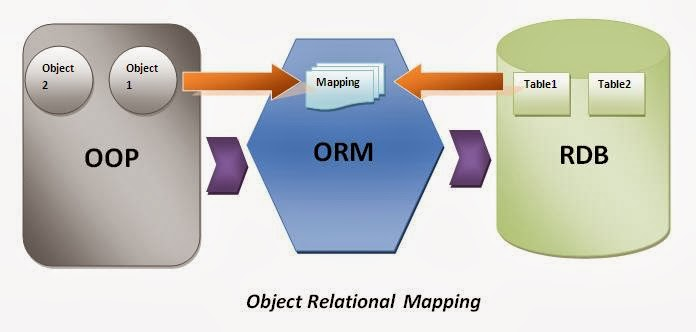
\includegraphics[width=\linewidth]{./orm1.JPG}
  \caption{ORM}
  \label{fig:ORM}
\end{figure}

\section{ORM vs Raw SQL}
Developers can use raw SQL code to write a direct interface between the application and the database. Most relational databases support SQL to build data interfaces and applications. It’s stable, and since SQL has been used since the 1970s, it’s well documented and supported. Programmers maintain a lot of control over their data interface with SQL. It requires a lot of work, but it is more flexible and detailed than an ORM abstraction.
\subsection{Native Querying with SQL}
\item Using raw SQL also has its drawbacks. For instance, the developer is responsible for the safety and security of the database code. SQL injection is a problem where user input can affect the data state causing issues with the application and data integrity. ORMs sanitizes the code, making it easier to avoid these problems.
\subsection{SQL Query Builders}
\item Query builders add a layer of abstraction over the raw SQL without masking all of the underlying details. The builders formalize querying patterns and add methods to or functions that add escape items for easier application integration. They add a templating layer to help developers understand the database structure within the same coding application. Template builders still require developers to understand the database structure, requiring them to know SQL.
\begin{figure}
  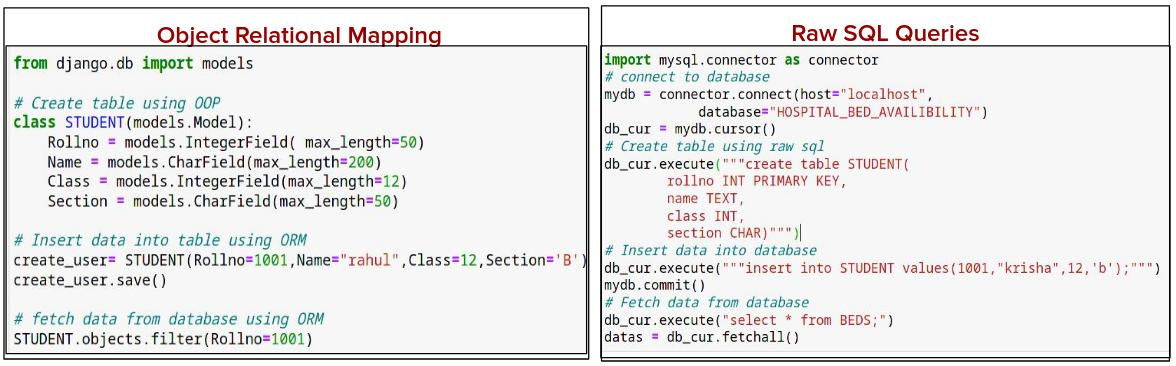
\includegraphics[width=\linewidth]{./orm2.JPG}
  \caption{ORM vs Raw SQL}
  \label{fig:ORM vs SQL}
\end{figure}


\section{Mapping Strategy Semantics}
\item


\section{Pros of ORM}
\item ORM tools are popular with OOP developers because they minimize the amount of SQL knowledge required to connect a database to an application. ORMs also automatically generate the SQL code, allowing you to focus on generating business logic. There are four significant benefits of using object-related mappers to manage the interface between applications and databases.
\subsection{Productivity}
\item Writing data-access code is time-consuming and doesn’t add a lot of value to the application’s functionality. It’s essentially the plumbing of the code. Using a tool like an ORM that automatically generates the data-access code saves tremendous development time that does not add value to the application. In some cases, the ORM can write 100 percent of the data-access code for the application. The ORM can also help you keep track of database changes making it easier to debug and change the application in the future.
\subsection{Application Design}
\item A well-written ORM will implement design patterns to force you to use best practices for application design. If you use an ORM to manage the data interface, you do not need to create the perfect database schema in advance. You will be able to change the existing interface easily. Separating the database table from the programming code also allows you to switch out data for different applications.
\subsection{Code Reuse}
\item One way to reuse data is to create a class library to generate a separate dynamic-link library (DLL). You can create a new application without needing to duplicate the data-access code.
\subsection{Reduced Testing}
\item Since the code generated by the ORM is well-tested, you do not need to spend as much time testing the data-access code. Instead, you can focus on testing the business logic and code.


\section{Cons of ORM}
\item ORMs are an excellent tool for many applications, but some developers found several drawbacks in using ORMs for data-access applications. The issues seem to correlate with the complexity of the application. With simple applications, having a high-level of abstraction helps the development process. But when the applications are complex, abstraction covers up many details needed to address data-related issues.
\subsection{Performance}
\item A common complaint among OOP developers is the extra code generated by the ORM. The added code slows application performance and makes it harder to maintain. A well-designed ORM should be able to create high-quality code without affecting application speed.
\subsection{Need to Know SQL}
\item High-level abstractions do not always generate the best SQL code, and developers cannot rely on the ORM 100 percent of the time. You still need to know SQL as well as the syntax generated by the ORM.
\subsection{Poor Mapping}
\item ORMs can sometimes create an incorrect mapping between data tables and objects. These problems can cause application problems and be difficult to recognize. ORMs also encourage one-to-one mapping even though it is rare that business applications have many one-to-one relationships.


\section{Conclusion}
Writing SQL code to attach a relational database to an object-oriented application can be a time-consuming activity that generates little value to the business application. Developers can write raw SQL code or use SQL query builders to improve the process, but both methods still require in-depth database knowledge and the ability to code in SQL. ORMs enhance productivity by creating highly-abstract data models and automatically generating SQL code. These tools also make it easier to separate the database from the programming logic giving developers more flexibility. But ORMs have their detractors. Common complaints include reduced performance, extra coding, and poor mapping depending on the ORM quality.


\section{Reference}
\begin{enumerate}
\item https://www.altexsoft.com/blog/object-relational-mapping/
\item file:///home/bhavin/Desktop/paper0605.pdf 
\end{enumerate}


\end{document}
